\section{Aviation climate impact mitigation}
\label{Mitigation}
It is customary practice among aviation policymakers to solely focus on mitigating the greenhouse effect induced by aviation carbon emissions. This means that analysis of the climate impact of non-\ce{CO_2} emissions is largely neglected, despite being responsible for over two-thirds of aviation-induced climate change \cite{Lee2021}. 

\subsection{Conventional \ce{CO2}-centric mitigation approach}
The industry fixation on aviation \ce{CO_2} mitigation stems from the easily quantifiable nature of the substance and its impacts; the direct coupling to fuel consumption and its relative stability and long lifetime make it a prime target for mitigation. This is due to the mutually assured reduction in both fuel consumption and corresponding \ce{CO_2} emissions, providing an economic and environmental incentive. Conventional mitigation approaches have often taken the form of improvements to aircraft and engine design, aviation technology and infrastructure, and aircraft operations, all aimed at minimising aircraft fuel consumption. These changes have been largely incremental due to the prioritisation of safety and economic stability over rapid implementation. As a result, efficiency gains have stalled in recent years (1--2\% per annum), whilst growth rates continue to rise unabated (4--5\% per annum) \cite{Peeters2016, Lee2021}. See figure \ref{eff_vs_growth} for a graphical representation of the trend in efficiency gains and aviation growth since 1940.

\begin{figure}[H]
	\centering
	\subfloat
		{
		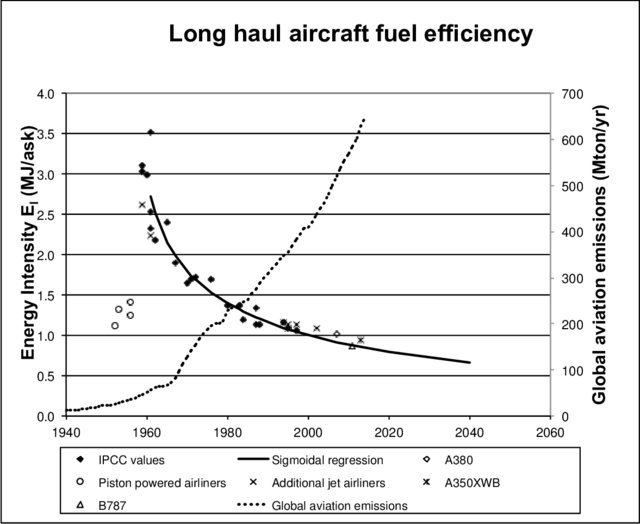
\includegraphics[width=.4\textwidth]{eff_vs_growth.jpg}
		%\vspace{.2cm}
		\label{eff_vs_growth}
		}
	\subfloat
		{
		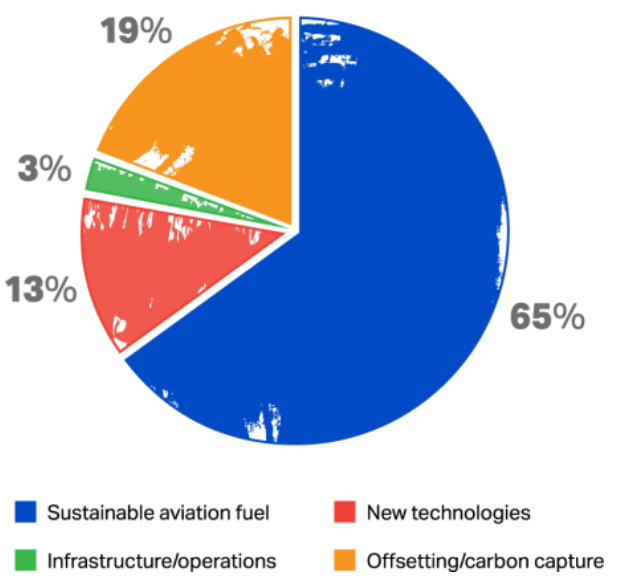
\includegraphics[width=.33\textwidth]{IATANetZero.png}
		\label{IATANetZero}
		}
	\caption{\textbf{(a)} Efficiency gains versus absolute aviation emissions growth since 1940 and projected to 2040 \cite{Peeters2016}. \textbf{(b)} IATA Net Zero 2050 contributions \cite{IATANetZero}.}
	\label{}
\end{figure}

At the International Air Transport Association (IATA) 77\textsuperscript{th} Annual General Meeting in 2021, a resolution was approved for the global air transport industry to achieve net zero carbon emissions by 2050, in accordance with the Paris climate agreement to limit global temperature rise to 1.5~\textdegree C \cite{IATANetZero}. This plan relies on the following contributions, as displayed in figure \ref{IATANetZero}: sustainable aviation fuels (SAFs) are to provide 65\% of the net carbon reduction, offsetting schemes and carbon capture are to deliver 19\%, new technologies such as hydrogen and electric propulsion to provide 13\%, and infrastructure/operational improvements to provide the final 3\%. This means that 78\% of the prospective net carbon emissions reduction comes from SAFs and alternative technology such as hydrogen and electric propulsion concepts. 

The fundamental issue with reliance on SAFs and nascent technologies, is that they may take decades to bring about noteworthy reductions in aviation climate impact. This is due to the need for a fleet-wide overhaul of aircraft equipment and associated ground infrastructure, which would likely incur huge costs and require extensive certification and approval processes \cite{ICF2021}. Not to mention, the environmental and ethical concerns have cast doubts over the prospect of a 4000 fold increase in global SAF production, to meet the IATA net zero target of 449 billion litres per year by 2050 \cite{IATANetZero, Henoi2022}. 

Carbon offsetting schemes, such as ICAO's Carbon Offsetting and Reduction Scheme for International Aviation (CORSIA), have been proposed to alleviate aviation climate impact in the meantime. However, an EU study investigating the efficacy of carbon offsetting indicates that such schemes often fall far short on providing meaningful mitigation, because of questionable offset quality, perverse incentives taking away from the real need to decarbonise, a lack of participation from key markets, and a clear lack of overall transparency and enforceability \cite{TandE2021, TandE2020}.

The remaining net zero contribution is expected to come from improvements to operations and infrastructure, which will continually provide 1--2\% per year. This will involve transitioning towards more efficient fuel management systems and improving overall technology and design of the aircraft, as well as advancing air traffic management systems and airspace modernisation \cite{Peeters2016}. However, as mentioned previously, improvements aimed at increasing aircraft fuel efficiency are largely outpaced by growth rates in passenger demand and hence emissions. Therefore, more must be done in the short term (i.e. the next 5 to 10 years), to reduce the dependency on nascent technologies which are still decades away from being impactful.

Whilst the proposed net zero targets are solely focused on decarbonising the aviation sector, it is inherently assumed that the reduction in non-\ce{CO_2} emissions will follow a similar trend. This review paper has evidenced however that this is not necessarily the case, due to the sensitivity of non-\ce{CO_2} emissions to combustor conditions, as well as the dependency of the atmospheric response on the environmental conditions of the ambient air. For this reason, action must be taken simultaneously to tackle non-\ce{CO_2} climate impact, alongside the current decarbonisation plan. with the potential to provide substantial climate impact reductions on a much shorter timescale.


%Global SAF production is currently only capable of providing ~0.05\% of total aviation fuel demand \cite{}, with a 4000 fold increase required to meet the net zero 2050 target \cite{IATA2050}. The prospect of upscaling SAF production at such a rapid rate has been overshadowed by feedstock supply and cost limitations, brought about by sustainability and ethical issues. This is due to the production of typical SAF feedstocks being (directly or indirectly) linked to ecosystem and biodiversity destruction, as well as detrimental impacts to low income and Indigenous communities, as reported in a landmark case study on the Omega Green refinery plant in Paraguay \cite{Henoi2022}. 


%Alternatively, the industry has looked towards longer term mass mitigation measures such as the implementation of sustainable aviation fuels (SAFs) and low carbon propulsion concepts such as hydrogen- or electric-powered flight. SAFs are renewable or waste-derived fuels that meet specific sustainability criteria laid out in ICAO Annex 16 Vol. IV \cite{Annex16}. These fuels typically have lower life-cycle \ce{CO_2} emissions of up to 70\% \cite{}, and also reduced PM emissions of soot and sulphate by 50-70\%, leading to alleviated contrail warming effects \cite{EASA2020, Voigt2021}. Such benefits are however, overshadowed by feedstock supply and cost limitations, which are largely brought about by issues related to sustainability and ethics. A recent landmark case study on the Omega Green refinery plant in Paraguay shed light on the tendency for typical SAF feedstocks to be directly or indirectly linked to ecosystem and biodiversity destruction and induces serious negative impacts on the local population, especially low income and indigenous communities \cite{Henoi2022}. Such findings cast doubt on the potential for the industry to increase SAF production by 4000 fold in the next 30 years, to achieve its contribution to the International Air Transport Association (IATA) Net Zero 2050 pathway \cite{IATAFlyNetZero}.

% Specify that elec and (green) hydrogen are best prospects for future low carbon flight
% Elec more suitable for short haul (find limitations and range) and hydrogen more for mid to long haul routes.
% EIS dates.
% Infrastructure and equipment overhaul and significant investment required to bring to fruition - IPCC need to begin decarbonising right now!

%Based on recent research relating to the need for developed nations to decarbonise fully by 2034 to retain a prospect of 50:50 chance of remaining within the 1.5°C emissions budget \cite{}, sole reliance on a low-carbon fuels strategy to mitigate UK aviation emissions is insufficient. As such, additional mitigation measures must be incorporated into the strategy in the interim to promote fleet-wide low-carbon flight. This is to increase the likelihood of limiting aviation’s climate contribution to 1.5°C, or at least below 2°C. 

\subsection{Alternative non-\ce{CO_2}-focused mitigation approach}
There are myriad solutions to mitigating aviation climate impact in the interim to low-carbon flight, however the focus here will remain on near-term operational mitigation measures that optimise aircraft routing by minimising non carbon-based radiative effects. 

As alluded to in sections \ref{emissions} and \ref{climate}, non-\ce{CO_2} emissions are on the other hand, produced in varying quantities depending on combustor conditions. Also, when released into the atmosphere, they have a spatio-temporally sensitive climate response, which depends on the background atmospheric conditions into which they are emitted. As such, anthropogenic as well as natural perturbations to atmospheric chemistry need to be considered; the entrainment of emissions to the exhaust plume for several hours post emission, leads to locally elevated emissions concentrations. This causes reactive non-\ce{CO_2} species to experience nonlinear chemical and microphysical processing that occurs at the scale of the plume, which subsequently affects their net climatic response when propagated to global scales.

Measures such as climate-optimal aircraft routing and formation flight present the potential for a substantial climate impact reduction in a relatively short timeframe, whilst requiring minimal technology changes to the current fleet and ground infrastructure.


\subsubsection{Climate-optimal aircraft routing}
The first measure proposed to tackle aviation’s non carbon-based environmental impact is climate-optimal aircraft routing. This involves re-routing aircraft in flight to avoid regions of the atmosphere that are particularly sensitive to non-\ce{CO_2} climatic effects, such as where \ce{NO_x} gives rise to excessive ozone production or where persistent contrails are formed. Simulation efforts have suggested that this method has the potential to reduce aviation climate impact by 10-20\%, at the cost of only a few percent of additional fuel consumption \cite{Grewe2014, Luhrs2016, Niklass2019a}. Moreover, the non-\ce{CO_2} climate impact from aviation is not evenly distributed across all flight distances, meaning that operational mitigation can be targeted towards flights which induce the most significant impact. For example, in a case study on contrail avoidance strategy \cite{Teoh2020}, it was found that diverting 1.7\% of the aircraft fleet could reduce the contrail climate impact by 59.3\%, with only a 0.014\% increase in fuel burn and accompanying additional \ce{CO_2} emissions. This sheds light on the sheer potential for significant reduction in aviation climate impact, through a minimally invasive climate-focused route optimisation strategy.

\begin{figure}[H]
  \centering
  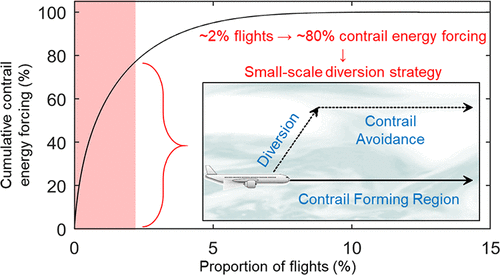
\includegraphics[width=0.7\linewidth]{Teoh.png}
  \caption{Schematic representation of contrail avoidance strategy. Plot of cumulative contrail energy forcing against proportion of flights \cite{Teoh2020}.}
  \label{Teoh}
\end{figure}

Implementation of this method in the real world does however require a number of issues to be addressed; Grewe et al. (2017) \cite{Grewe2017} lay out four key hurdles that must be overcome: 

\begin{enumerate}
	\item The accuracy and robustness in determining eco-efficient flight trajectories must be improved, and this must be possible near real time.
	\item Consensus must be achieved on determining the extent to which cooling effects should be exploited (e.g.\ intentionally flying a route that generates a cooling contrail could be seen as unnecessary intervention in nature).
	\item The implications of fleet-wide climate-optimal routing on the air traffic management system must be assessed rigorously, to ensure safety, order and efficiency is maintained.
	\item A non-CO2 market-based measure or policy pathway must be adopted to incentivise this transition towards a climate-optimised air traffic network.
\end{enumerate}

In the time since, a dedicated network of researchers from various institutions have been working towards bringing this concept to fruition on a large scale. The FlyATM4E research group has been developing methodologies to increase robustness in the determination of eco-efficient flight trajectories using so-called algorithmic climate change functions (aCCFs) \cite{Matthes2020}. Live trials are currently ongoing in the Maastricht Upper Area Control (MUAC) to investigate the operational feasibility of contrail prevention from an air traffic control perspective \cite{MUAC2021}. The inclusion of non-\ce{CO_2} effects of aviation in the European Union emissions trading scheme (EU ETS) and under CORSIA has also been discussed in great detail in a comprehensive report by Nikla{\ss} et al. (2019b) \cite{Niklass2019b}. Most recently, a comprehensive survey paper was published by Simorgh et al.\ (2022) \cite{Simorgh2022}, detailing the current operational strategies that are proposed in the state-of-the-art literature published in this field over the last few decades. The aim of this review was to collate methodologies used for aircraft performance modelling, climate modelling and optimisation, and to identify gaps to guide future research.

%Newinger and Burkhardt (2012) \cite{Newinger2012} explored the potential for mitigation of nighttime contrail forcing through air traffic scheduling adjustments. They proposed...


%Mention alt fuels, alt propulsion, technological changes etc. and say how they are long term due to infrastructure overhaul and large investment. Operational mitigation strategies require minimal change to current system, only operational changes which can be implemented without much additional investment. Just need more research and 

\subsubsection{Formation flight}
\label{Formation_flight}
Formation flight for wake energy retrieval involves the flight of two or more aircraft, with the follower aircraft positioned in the smooth updraft of the leader aircraft’s wake. This has been demonstrated in simulation \cite{Venkataramanan2003, Bangash2004} and flight testing \cite{Hanson2002} to reduce required lift and thrust of the trailing aircraft and offer a 5--10\% reduction in fuel burn in paired formation. Most work to date focuses on two-aircraft configurations, however three \cite{Bower2009} and more have also been considered. In figure \ref{Marks}, it is evident how this concept is used in practice to obtain aerodynamic benefits. The counter-rotation of the wake vortices of the leader aircraft leads to a stream of upwash on the outside of either rolled up vortex. Flying a follower aircraft in this region of upwash induces a vertical velocity, with aerodynamic benefits achieved at distances as much as 30 wingspans (i.e. \textasciitilde1~km for Airbus A320).

Safety is a critical hurdle, particularly in close formation cases, along with regulatory and air traffic systems and processes. Airbus' fello’fly wake energy retrieval project has undertaken initial work to identify and address operational and safety challenges, proposing regulatory standard adaptations to facilitate adoption, and conducting a trial transatlantic flight in 2021 \cite{Airbus2021}. Claims in this document state that formation flight strategies could be deployed around the middle of this decade. Proposed longitudinal separation distances for formation flight range from 56~ft \cite{Hanson2002} to 1.5~NM \cite{Airbus2021}, with lateral distances ranging from 10\%-span overlap to 30~m separation showing benefit. Routing aircraft into formation has been considered in simulation \cite{Xu2014}, with net fuel (and hence \ce{CO_2} saving benefits of 5.8\% being identified for a single operator, rising to 7.7\% for a transatlantic alliance. Significant benefits have been projected for long-haul and transatlantic routes, with more modest reductions for low-cost airline cases \cite{Kent2020}. 

% How many aircraft in transatlantic alliance??

\begin{figure}[H]
  \centering
  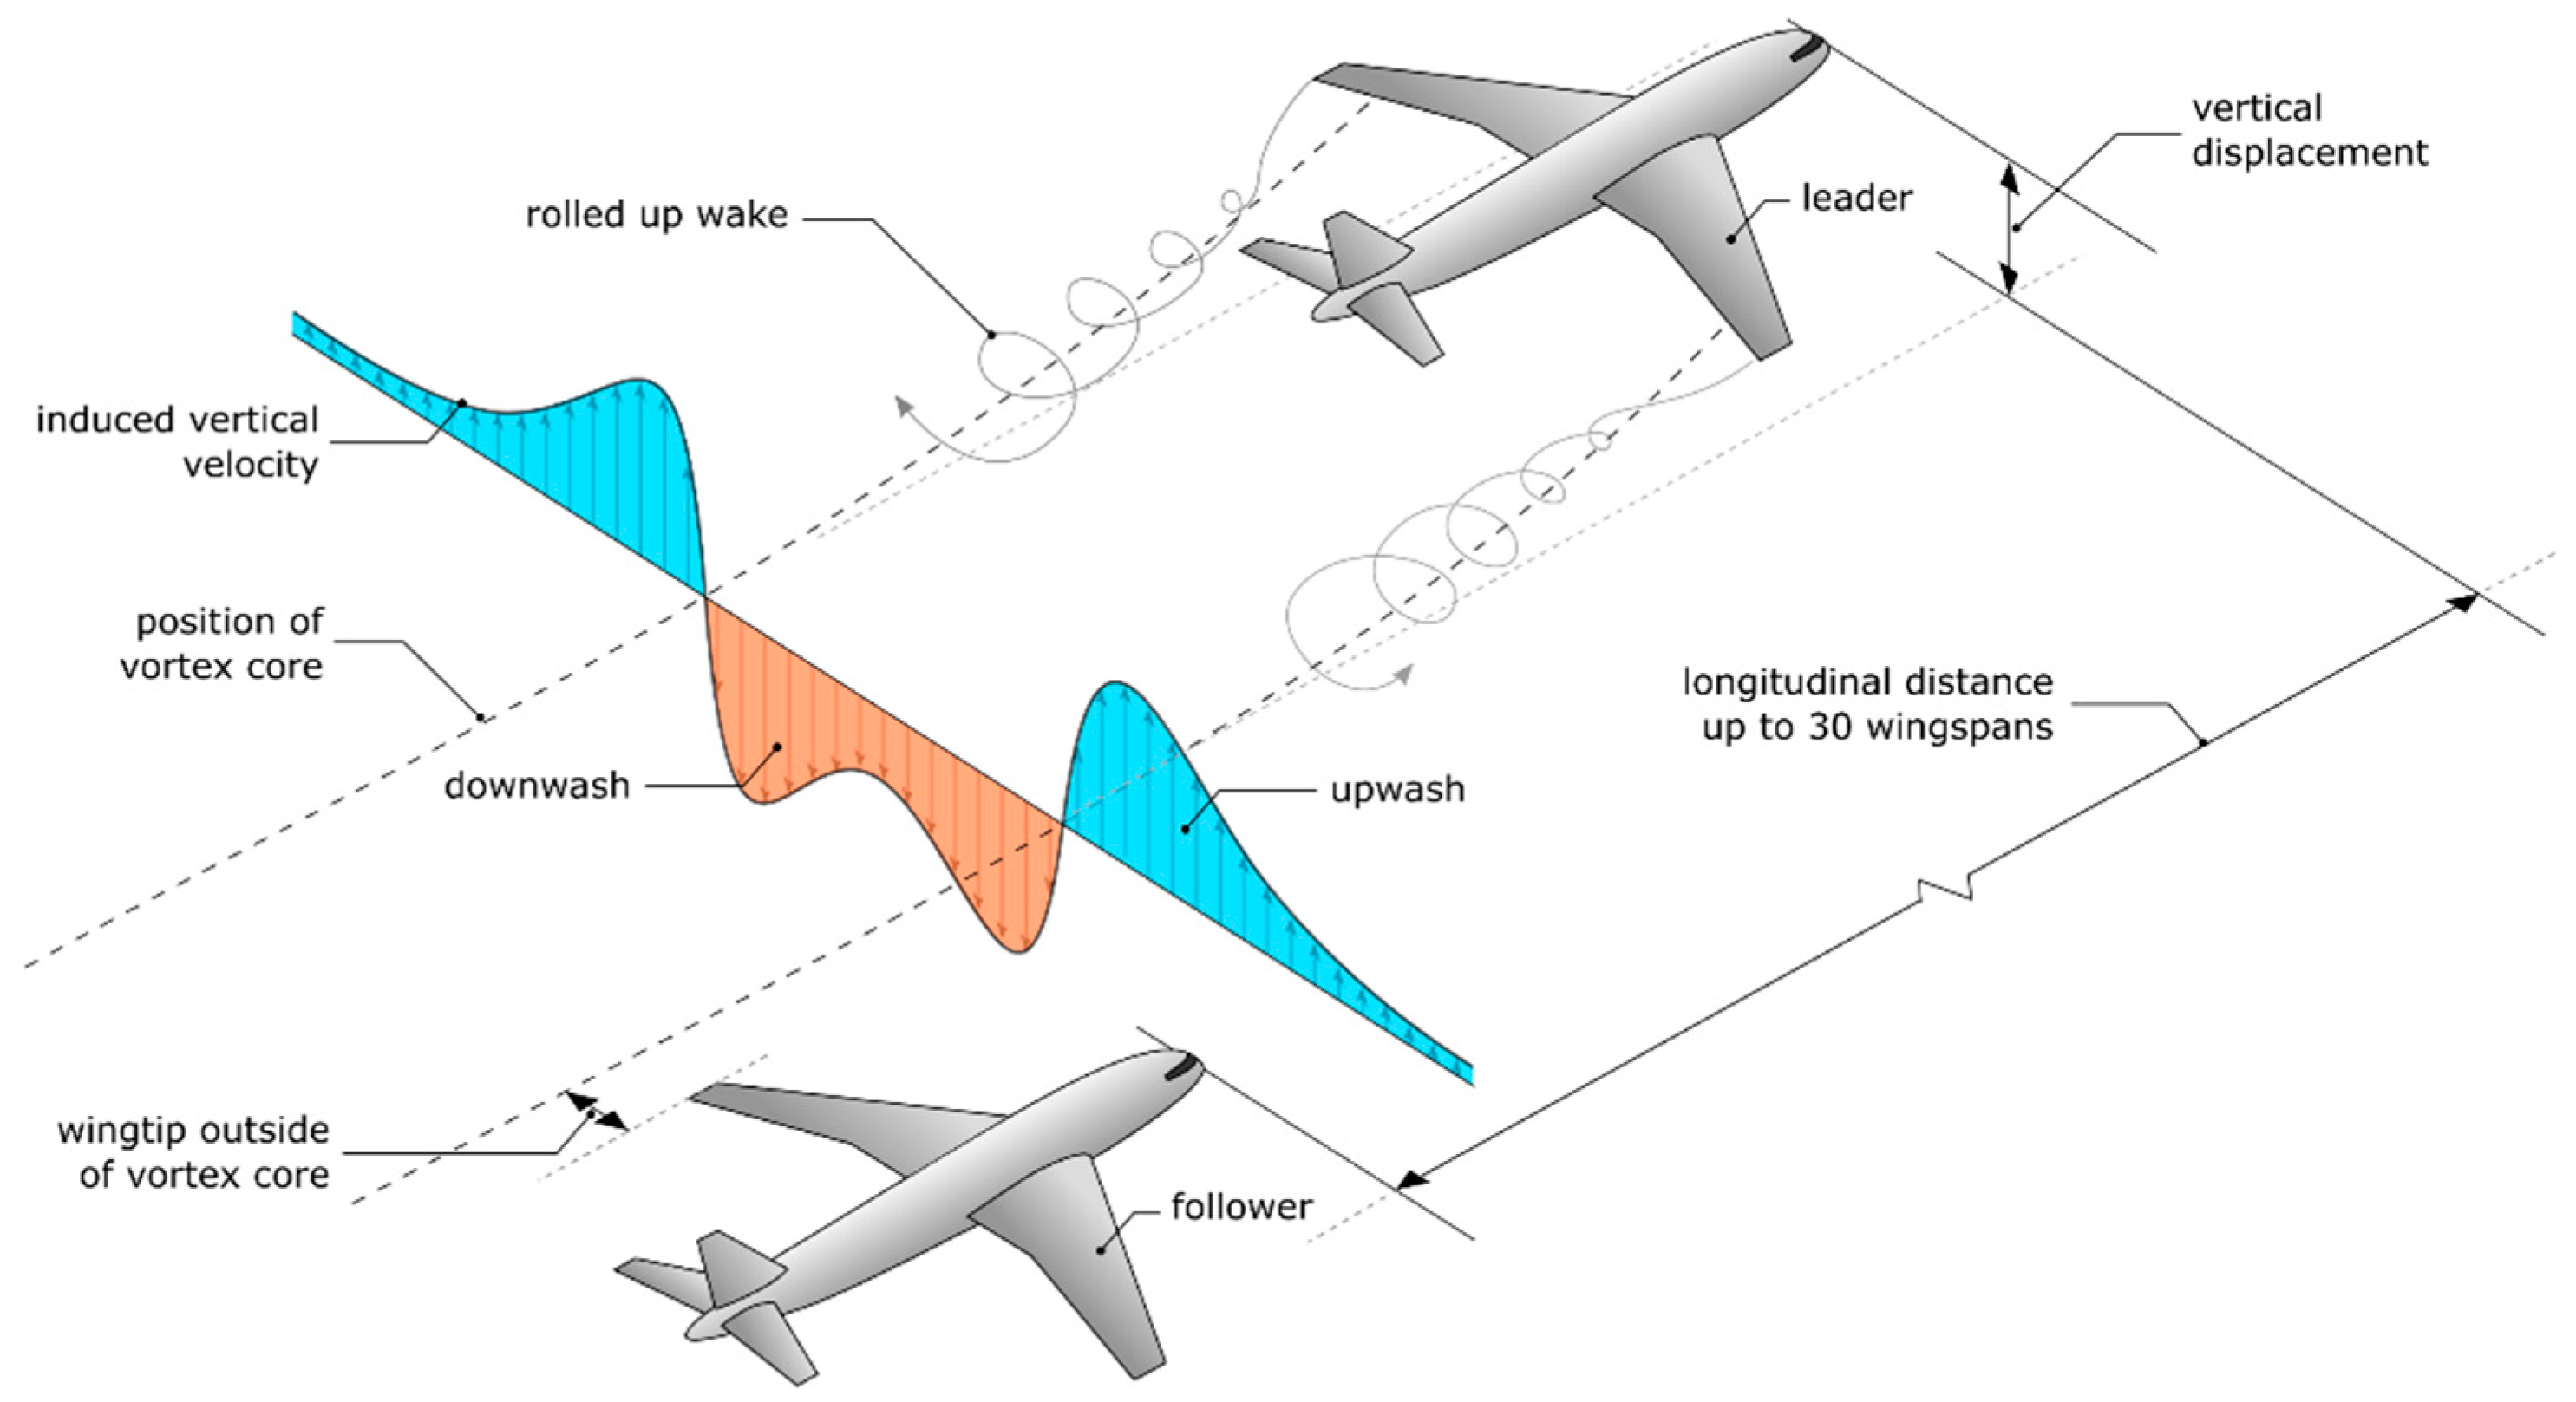
\includegraphics[width=0.8\linewidth]{FF.png}
  \caption{Visual representation of the formation flight concept, depicting the fundamental principles of wake energy retrieval \cite{Marks2020}.}
  \label{Marks}
\end{figure}

Non-\ce{CO_2} impacts have been neglected until recently, but a synergistic outcome of formation flight is realised via the saturation of emissions in the trailing exhaust plumes, leading to the aforementioned nonlinear chemical and microphysical response that reduces ozone and contrail formation, as detailed in section \ref{Saturation}. This has been projected to offer net climate impact reduction for a two-aircraft formation of 13--33\% \cite{Dahlmann2020}, which is significantly higher than the \ce{CO_2}-focused formation discount factors employed in the routing simulations mentioned above. Given the near-term feasibility demonstrated in industry-led trials, and the combined \ce{CO_2} and non-\ce{CO_2} benefits that produce an outsized impact when overall ERF is considered, formation flight offers a promising interim solution that can continue to be employed for drag reduction/wake energy retrieval once SAFs and hydrogen/electric propulsion are more widespread.

In this section, the prospects of non carbon-based operational mitigation measures have been discussed, and their potential to reduce aviation's net climate impact has been investigated. Gradual efficiency gains are unable to outpace the rapid growth in demand year upon year, meaning that more radical approaches must be implemented in order to achieve net zero emissions targets. For this reason, two concepts have been proposed and discussed: climate-optimal aircraft routing and formation flight. The former aims to re-route the aircraft to minimise time spent in particularly climate sensitive regions of the atmosphere, whereas the latter aims to optimise atmospheric conditions artificially by overlapping aircraft plumes and saturating local concentrations of emissions to lead to climate-beneficial effects. For the industry to truly reap the benefits and maximise potential non-\ce{CO_2} reductions from implementation of these measures, there is the potential to perform them simultaneously, in a controlled and safe manner. This would involve flying aircraft in formation, along routes which are optimised with respect to minimum climate impact.  





%Formation flight involves the flight of two or more aircraft in aerodynamic formation, with the follower aircraft positioned in the smooth updraft of the leader aircraft’s wake, reducing required lift and thrust, hence reducing fuel and CO2 emissions by 5-8\% per trip \ref{}. A fortuitous outcome of formation flight is however, the saturation of emissions in the trailing exhaust plumes, which can lead to the aforementioned nonlinear chemical and microphysical response that reduces ozone and contrail formation. The non-CO2 climate effects of a twin-aircraft formation flight are observed in \ref{}, where a climate model was used to determine the changes in NOx-related ozone production and contrail formation processes. The case study found that, despite a 1-3\% increase in flown distance, CO2 was reduced by 6\% and NOx was reduced by 11\%. This resulted in a 5\% reduction in ozone production efficiency due to NOx  saturation and a 48\% contrail reduction due to mutual competition for available water vapour, resulting in a total climate impact reduction of approximately 23\%. While part of the alleviated climate impact can be related to the decrease in total emissions due to wake energy retrieval of the follower aircraft, there is also further emphasis due to the saturation of emissions in the overlapping plumes of both aircraft involved. This demonstrates great potential for reducing both CO2- and non-CO2-induced climate effects from aviation, if such a scheme were to be carried out on a global scale.

%\subsubsection{Climate-optimal aircraft routing}
%Fleet-wide implementation of formation flight would however, pose a number of research obstacles, that must be overcome to maximise its cost-benefit potential, whilst ensuring the safe and orderly operation of aircraft in controlled airspace. Optimising aircraft trajectories to minimise fuel burn requires the consideration of nonlinear aircraft performance, wind and weather, payload, fuel load, and constraints set out by air traffic control \cite{}. Formation flight adds another variable to the fuel burn optimisation problem, maximising the time spent flying in formation whilst minimising deviation from the true optimal route. This is a research topic covered extensively in the literature \cite{}. Optimising formation flight trajectories to minimise climate impact on the other hand, is a relatively novel concept, which requires deeper understanding of the sensitivity of the climate response to emissions under a range of different atmospheric states. 



%Optimising a flight to minimise fuel burn very rarely results in minimum climate impact. This is because of the presence of climate-sensitive regions of the atmosphere where aircraft emissions have a higher climate impact per 

%\subsection{Alternative propulsion technologies}
%In recent years, new aircraft propulsion systems are being developed to operate on alternative aviation fuels (e.g. bio-jet fuels, electric, hybrid electric, hydrogen) which can significantly reduce both the CO2 and non-CO2 emissions from aviation sector (Voskuijl et al., 2018; Schafer et al., 2019). However, it is important to understand the technical, environmental and economic performance of these alternative fuels and the subsequent propulsion technologies for the broad application of these fuels. 